\documentclass[12pt]{article}

\usepackage{graphicx}
\usepackage{endfloat}
\usepackage{amssymb}

%% THE NEXT TWO LINES INSERT THE PACKAGES FOR JASA FORMAT:
\usepackage[abbr]{jasa_harvard}    % 	for formatting citations in text
\usepackage{JABES_manu}

%% CHANGING THE 'AND' IN THE HARVARD BIBLIOGRAPHY PACKAGE TO WHAT IT OUGHT TO BE
\renewcommand{\harvardand}{and}

\usepackage{rotating}

\DeclareDelayedFloatFlavor{sidewaysfigure}{figure}
\DeclareDelayedFloatFlavor{sidewaystable}{table}

\begin{document}

\title{Confidence Intervals for Run Composition \\ of Returning Salmonids}
\author{Kirk Steinhorst, Timothy Copeland, Mike Ackerman, Bill Schrader, and Eric Anderson 
}
\maketitle

\footnote{Kirk Steinhorst is Professor Emeritus, Department of Statistical Science, University of Idaho, Moscow, ID 83844-1104 (E-mail: mailto:kirk@uidaho.edu). Timothy Copeland is Senior Fishery Research Biologist, Idaho Fish and Game, Nampa, ID 83686. Mike Ackerman is Fishery Research Biologist, Pacific States Marine Fisheries Commission \& Idaho Department of Fish and Game, Eagle Fish Genetics Lab, Eagle, ID 83616. Bill Schrader is Principal Fishery Research Biologist, Idaho Fish and Game, Nampa, ID 83686. Eric Anderson is Research Molecular Geneticist, Fisheries Ecology Division, Southwest Fisheries Science Center, Santa Cruz, CA 95060}

%% ABSTRACT

\newpage
\begin{center}
\textbf{Abstract}
\end{center}
We propose weighted estimators of fish composition for wild steelhead and Chinook salmon returning to a single point in a river system.  Using data on overall fish numbers derived from counts at an observation window, trap data providing separation of wild and hatchery fish, and compositional data on sex, age, and genetic stock of wild fish, we propose one-at-a-time and simultaneous confidence intervals for numbers by sex or age or stock based on parametric bootstraps of both the wild/hatchery data and the sex/age/stock data.  Using two simulations, we show that the estimators are generally unbiased with confidence intervals that have good coverage.  Depending on the size of the group, we know the true numbers within 10\%, 25\%, or 50\%.

\vspace*{.3in}

\noindent\textsc{Keywords}: {Bootstrap, Stratified Sampling, Salmonid Escapement, Simultaneous Inference}

\newpage

\section{Introduction}
Migratory life histories are important in fisheries management and conservation  \cite{Hilborn1992,McDowall2009}. Given migratory characteristics, the spatial distribution of a stock or population is predictable, which facilitates exploitation and also sampling for research and management. Sampling may be conducted by test fisheries (e.g., \citeasnoun{Flynn2004},\citeasnoun{Beacham2012}), hydroacoustics (e.g., \citeasnoun{Tarbox1996}, \citeasnoun{Pritt2013}), or by other means. A highly controlled sampling regime can be instituted by counting or sampling fish as they move past barriers such as weirs or dams (e.g., \citeasnoun{Wagner2007}). In all of these sampling scenarios it is typical to subdivide overall abundance into groups of management interest by applying compositional data (e.g., species, stock, age, and sex) derived either from the primary sampling gear or by a secondary sampling gear (e.g., using gill net samples to allocate hydroacoustic counts to species, \citeasnoun{Rudstam2012}). The complexities of fisheries sampling programs and the relevant groups into which the fish are parsed present difficulties for estimating precision about the point estimates generated.

There are two approaches to determining run composition \cite{Starr1988}: 1) Direct identification of fish from tags, scales, genetic analysis, and/or morphology and 2) Reconstruction of the run from catch data, adult escapement numbers (numbers of fish returning from the ocean to a given point), and migration paths \cite{Buckland2007,Newman2009,Branch2010}.  Run reconstruction uses maximum likelihood estimation of a product of probability density functions describing arrivals, escapement, harvest, and ages or it uses state-space models and Bayesian estimation via MCMC. Bayesian intervals provide information on precision of estimates.

There is no statistical literature on properties of estimators and confidence intervals for composition determined from direct identification. This paper provides a statistical evaluation of estimators derived for use with data collected via direct identification methods. We observe adult steelhead \textit{Oncorhynchus mykiss} and Chinook salmon \textit{O. tshawytscha} as they migrate past Lower Granite Dam (LGD) on the Snake River 695 kilometers from the ocean. Adults returning from the Pacific Ocean to spawn in tributaries of the Snake River must ascend fish ladders at eight dams during their migration including four on the Columbia River and four on the Snake River. LGD is the final dam they encounter on the Snake River; fish migrating past LGD then disperse to tributaries throughout the Snake River basin to spawn. An observation window on the LGD fish ladder allows us to count fish by species as they migrate upstream.  A trapping facility located above the observation window allows us to intercept fish as they migrate past and collect data and obtain biological samples.  The counting and sampling of returning adult steelhead and Chinook salmon at the dam provides direct data for calculating composition \cite{Harmon2003,Steinhorst2010,Schrader2013}.

Steelhead trout and Chinook Salmon are a critically important resource in the Pacific Northwest; both species are culturally, economically, and recreationally valuable. Following the construction of hydroelectric dams on the Columbia and Snake rivers during the late 1960s and early 1970s, the abundance and survival of steelhead and spring-summer run Chinook salmon in the Snake River decreased \cite{Raymond88}. In response, both species within the Snake River basin were listed as threatened under the Endangered Species Act (ESA) in the 1990s. In recent years, abundances have increased slightly. However, the increase has been dominated by fish produced in hatcheries (intended to mitigate for lost fisheries and to supplement natural populations), while the returns of steelhead and Chinook salmon born in the natural environment remain critically low \cite{Busby1996}. Fisheries biologists need to know how many wild versus hatchery steelhead and salmon return in order to properly manage fisheries as well as to assess the conservation status of wild populations. Further, for wild fish, we want to know numbers of fish returning by sex, age, and genetic stock.

\citeasnoun{McElhany2000} in a document published by the National Oceanic and Atmospheric Administration (NOAA), provide guidance for status and trends monitoring of ESA-listed Pacific salmon populations based on Viable Salmonid Population (VSP) indicators. VSP indicators include adult spawner abundance, productivity, spatial distribution, and diversity. NOAA recommends unbiased abundance estimates with a coefficient of variation (CV) of 15\% or less \cite{Crawford2011}. For a 90\% asymptotic confidence interval, it follows that $ |\hat{N}-N|\le 1.645se\le 1.645(0.15)\hat{N}\le 0.25\hat{N}$ or $ |\hat{N}-N|/\hat{N}\le 0.25$, i.e., NOAA recommends that the estimate falls within 25\% of the truth. Researchers often set a more stringent goal of estimating the truth within 10\%.  For small groups, both of these sampling criteria may be too stringent.  If there are only a few fish in a category, one would probably be content with a more \underline{lenient} rule. For example, if our estimate is 50 and the confidence interval is (20, 80) then the percent half width is 60\% of the estimate. Knowing that the true number is between 20 and 80 might be sufficient especially if the numbers of fish in other groups are decidedly larger.

We examine the properties of estimators of composition and their confidence intervals derived from weightings of window counts, wild/hatchery data obtained from the trap samples, and sex/age/genetic stock compositional data collected on wild fish subsampled at the trap. We consider counts at the observational window to be a census of fish passing the dam. Thus the total number of fish returning to LGD is considered known.  One-at-a-time and simultaneous confidence intervals for subgroups are derived via a combination of bootstrap sampling of both the wild/hatchery trap data and the compositional data.  We are particularly interested in knowing if the estimators are unbiased and what precision can be expected as measured by half the confidence interval as a percentage of the estimate.

In section 2, we describe the setting and the data collection and processing methods. In section 3, we present the estimators and methods for obtaining the bootstrap confidence intervals. In section 4, we give the results for 2011 steelhead and salmon runs. Section 5 contains the results of simulations examining the properties of the estimators and confidence intervals.

\section{Data Collection}
This paper summarizes the abundance and composition of wild adult steelhead and spring/summer Chinook salmon migrating past LGD during spawn year (SY) 2011. For steelhead, the SY2011 run is defined as adults migrating past LGD between 07/01/10 and 06/30/11. While all steelhead in the Snake River basin spawn in the spring, the majority migrate past LGD during the previous fall, with a smaller portion migrating in the spring just prior to spawning. For spring/summer Chinook salmon, the SY2011 run is defined as adults migrating past LGD during the 2011 calendar year prior to 08/17/11. Spring/summer Chinook begin arriving at the dam in April. Chinook migrating past LGD after 08/17/11 are considered fall Chinook, a separate lineage of Chinook salmon.

Live window counts are conducted throughout a majority of the year and occur from 0400 to 2000 Pacific Time. Video counts are used in lieu of window counts in November, December, and March and occur from 0600-1600. Most fish pass the window during the 10 to 16 daylight hours when counts are made \cite{Cassinelli2012}. The ladder is closed in January and February. Count data were downloaded from the Corps of Engineers (COE) website: http://www.nwp.usace.army.mil/Missions/Environment/Fish/Data.aspx. The steelhead count consists of all fish $>$ 12'' identified as O. mykiss. For Chinook salmon, adults ($\geq$ 56 cm) and jacks (males that return after only one year of saltwater residency, 30-–56 cm) are counted separately; we combined the two counts to get total counts on a daily basis. Daily counts were aggregated on a weekly basis. Early and late in the season weeks were collapsed into longer strata if few fish were passing.

Trap sampling rates are determined by a committee of co-managers in order to achieve sample requirements for multiple projects and to balance fish handling concerns; sample rates are typically 10-–20\%. The sample rate determines how long a trap gate remains open four times per hour; the trap is operational 24 hours per day. Trapped fish are anesthetized and examined to determine whether they are of hatchery or wild origin. Scale and tissue samples are taken from a subsample of trapped fish determined to be wild. Scale samples are used to determine age based on visual examination of scale annuli (detailed methods in \citeasnoun{Schrader2013}). Age data collected at LGD are used to assign returning adults back to specific brood years.

Tissue samples for DNA extraction and single nucleotide polymorphism (SNP) genotyping were taken from a small clip of the anal fin.  Tissue samples are used to determine sex and estimate genetic stock of origin. The genetic stock of each fish is estimated using individual assignment (IA), a type of genetic stock identification  \cite{Pella1987,Shaklee1999}, using multi-locus SNP genotype data.  All adults queued for genotyping were screened at 191 SNPs and the sex-specific allelic discrimination assay \cite{Campbell2012}. IA allocates each fish to the population in which the probability of its genotype occurring is the greatest. IA was performed using the Bayesian version of the program gsi\_sim \cite{Anderson2008,Anderson2010}. For this study, we assumed that genetic stock could be determined without error (a future study will incorporate uncertainty in genetic assignments). 

\citeasnoun{Ackerman2014} defined the genetic stocks used for IA at LGD. Ten genetic stocks were defined for steelhead. Genetic stocks include: 1) UPSALM: the upper Salmon River; 2) MFSALM: Middle Fork Salmon River (including Chamberlain and Bargamin creeks); 3) SFSALM: South Fork Salmon River; 4) LOSALM: lower Salmon River; 5) UPCLWR: upper Clearwater River (Lochsa and Selway rivers); 6) SFCLWR: South Fork Clearwater River (including Clear Creek); 7) LOCLWR: lower Clearwater River; 8) IMNAHA: Imnaha River; 9) GRROND: Grande Ronde River; and 10) LSNAKE: Tucannon River, Asotin Creek and tributaries to the Snake River downstream of the Clearwater River confluence.

Seven genetic stocks were defined for Chinook salmon. Genetic stocks include: 1) UPSALM: upper Salmon River; 2) MFSALM: Middle Fork Salmon River; 3) CHMBLN: Chamberlain Creek; 4) SFSALM: South Fork Salmon River; 5) HELLSC: an aggregate stock that includes the Little Salmon, Clearwater, Grande Ronde, and Imnaha rivers and small tributaries of the Lower Snake River; 6) TUCANO: Tucannon River, and 7) FALL: Snake River fall Chinook salmon. The FALL genetic stock represents a separate lineage of Chinook salmon in the Snake River basin and is managed as a separate species under the ESA.

The above sampling design produces three datasets: 1) a census of fish numbers returning to and migrating past the dam (window counts), 2) a hatchery versus wild dataset for all trapped fish (trap data), and 3) a dataset containing sex, age, and stock for a subsample of wild fish that were trapped (compositional data). These three data sets are used to produce the size of the run and estimates and confidence intervals for number of fish by sex or age or genetic stock.

\section{Estimates and Confidence Intervals}
The proportions of wild and hatchery steelhead or salmon changes over the season, but within a week are relatively constant. Given weekly counts, \(C_1,C_2,...,C_n\),   the number of wild steelhead or salmon is estimated as
\[\hat{W}=\sum\limits_{h=1}^{n} \hat{p}_hC_h\]	  
where \(\hat{p}_1, \hat{p}_2, \ldots, \hat{p}_n \) are estimates of proportion wild by week from the trap data.  Since the window counts are assumed to be fixed, we find a confidence interval for the number of wild fish using a parametric  bootstrap to produce $B$ bootstrap sets of \((p^*_1, p^*_2, \ldots, p^*_n)\) yielding \(W^*_1, W^*_2, \ldots, W^*_B\).   That is, for week $h$ we assume the bootstrap number of wild fish has a binomial distribution,  \(T^*_h\sim binomial(n_h,\hat{p}_h|n_h)\) where \(n_h\)  is the number of fish trapped for that  week and \(p^*_h = T^*_h/n_h\).  The \(100\alpha/2-th\) and \(100(1- \alpha/2)th\) percentiles of \(W^*_1, W^*_2, \ldots, W^*_B\) give us the \(100(1-\alpha)\%\) confidence interval for the true number of wild steelhead or Chinook passing LGD for the year.

Define \(\pi_{Fh} = P(female|wild,week \: h)\).  Then we have \((\pi_{F1},\pi_{M1}),\ldots,(\pi_{Fn},\pi_{Mn})\) as the conditional probabilities for wild females and males for weeks \(1,\ldots,n\).  Similarly for $A$ ages, we have conditional probabilities \((\pi_{11}, \ldots, \pi_{A1}), \ldots,(\pi_{1n}, \ldots, \pi_{An})\). For $g$ stocks, we have conditional probabilities \((\pi_{11}, \ldots, \pi_{g1}), \ldots,(\pi_{1n}, \ldots, \pi_{gn})\). Given estimates of these probabilities from wild fish examined in the trap, we obtain  
\[\hat{F} =\sum\limits_{h=1}^{n}\hat{\pi}_{Fh}\hat{W}_h = \sum\limits_{h=1}^{n}\hat{\pi}_{Fh}\hat{p}_{h}C_h ~~~ \mathrm{and}  ~~~ \hat{M} =\sum\limits_{h=1}^{n}\hat{\pi}_{Mh}\hat{W}_h = \sum\limits_{h=1}^{n}\hat{\pi}_{Mh}\hat{p}_{h}C_h \]
and
\[\hat{N}_1 =\sum\limits_{h=1}^{n}\hat{\pi}_{1h}\hat{W}_h = \sum\limits_{h=1}^{n}\hat{\pi}_{1h}\hat{p}_{h}C_h, \ldots, \ \hat{N}_A =\sum\limits_{h=1}^{n}\hat{\pi}_{Ah}\hat{W}_h = \sum\limits_{h=1}^{n}\hat{\pi}_{Ah}\hat{p}_{h}C_{h}\]
and
\[\hat{N}_1 =\sum\limits_{h=1}^{n}\hat{\pi}_{1h}\hat{W}_h = \sum\limits_{h=1}^{n}\hat{\pi}_{1h}\hat{p}_{h}C_h, \ldots, \ \hat{N}_g =\sum\limits_{h=1}^{n}\hat{\pi}_{gh}\hat{W}_h = \sum\limits_{h=1}^{n}\hat{\pi}_{gh}\hat{p}_{h}C_{h}.\]
That is, the number of wild females or males is a weighted sum of the weekly window counts where the weights are estimates of the probability of being wild and female (or male).  Likewise for ages \(1, \ldots, A\) or genetic stock \(1, \ldots, g\), the estimate is a weighted sum of the weekly counts with weights that are an estimate of the probability of being wild of that age or genetic stock.

To find confidence intervals for these estimates we have to account for the variability of both the trap data and the compositional data.  We do this by extending the parametric bootstrap process used above for obtaining the confidence interval for number wild by adding a conditional parametric bootstrap based on the sex/age/stock of wild fish in the trap.

For sex, define pseudoreplicates using
\[(F^*_h,M^*_h) \sim binomial(m_h,(\hat{\pi}_{Fh},\hat{\pi}_{Mh})|m_h, wild) \ and \ (\pi^*_{Fh}=F^*_h/m_h,\pi^*_{Mh}=M^*_h/m_h) \]	  
where \(m_h\)  is the number of wild fish sexed during week $h$.  Bootstrap values for the number of wild females, \(F^*_1,\ldots, F^*_B, \) follow from \(F^*=\sum\limits_{h=1}^{n}\pi^*_{Fh} p^*_{h}C_h \).    The percentile bootstrap confidence interval for true number of wild females, \([L_F,U_F]\), is given by finding the \(100 \alpha/2-th\) and \(100(1-\alpha/2)th\) percentiles.  Similarly, we find a bootstrap confidence interval for the number of wild males.   Changing the binomial above to a multinomial, we generate $B$ sets of \((\pi^*_{11}, \ldots, \pi^*_{A1}), \ldots,(\pi^*_{1B}, \ldots, \pi^*_{AB})\) to obtain bootstrap confidence intervals for the true number of wild fish of ages 1,..., A. We follow the same procedure for genetic stocks $1,\ldots,g$.

Simultaneous confidence intervals for numbers of wild fish by sex or age or genetic origin are found using the methods of \citeasnoun{Mandel2008}. 

\section{Results for spawn year 2011}
\label{sec:results}

We consider two empirical examples to illustrate the methods outlined in section 3 –-- steelhead and Chinook salmon returning to spawn in 2011. A total of 208,296 steelhead were counted at LGD during SY2011. Of these, we estimate that 44,452 were wild (21.3\%, Table \ref{table:SHresults90}).  Based on B = 5,000 bootstrap iterations, the 90\% confidence interval is (43454,45473). We found 90\% one-at-a-time and simultaneous confidence intervals on the numbers of each sex, on numbers by age (brood year), and numbers by genetic stock. The simultaneous confidence intervals were found separately for sex, age, and stock. In addition to female and male, there are five ages, and ten genetic stocks for steelhead. The simultaneous confidence intervals are proportionally wider for age and stock than for sex. Columns P1 and Psim give half the width of the confidence interval as a percentage of the estimate. If the estimate is near the center of the confidence interval then we are 90\% confident that we know the truth within this percentage of the estimate. Confidence intervals for total wild, sex, BY05, BY06, BY07, GRROND, LSNAKE, and UPSALM meet our 10\% (researchers') goal for confidence interval width. BY04 and BY08 have percent half widths of 26.4\% and 33.1\% respectively, thus not meeting the 25\% sampling goal recommended by NOAA. The remaining genetic stocks are reasonably well estimated; the percent half widths fall in the range 10.4 to 15.2\%.

The percent half widths for the simultaneous confidence intervals for sex are under 10\%.  The percent half widths for BY04 and BY08 32.3\% and 39.1\% respectively. The remaining percent half widths are 21.9\% or less.

\begin{table}
\caption{Estimates and 90\% confidence intervals for steelhead}
\label{table:SHresults90} 
\begin{center}
\begin{tabular}{|l|r|r|r|r|r|r|r|r|}
\hline Group &n& Estimate & L & U & P1 & $L_{sim}$ & $U_{sim}$ & Psim \\ 
\hline  Wild&4707&44452  &43454  &45473  & 2.3  & & &  \\ 
\hline  F&1466&29698&28512&30984&4.2&28257&31264&5.1  \\
\hline  M&732&14754&13802&15735&6.6&13678&15877&7.5  \\
\hline  BY04&38&796&592&1011&26.4&558&1072&32.3  \\
\hline  BY05&520&11070&10344&11815&6.6&9761&12520&12.5  \\
\hline  BY06&994&21574&20602&22523&4.5&19440&23867&10.3  \\
\hline  BY07&473&10423&9699&11184&7.1&9152&11852&13.0  \\
\hline  BY08&26&589&406&796&33.1&383&844&39.1  \\
\hline  GRROND &405&8158 &7550 &8779 &7.5  &7068 &9378 &14.2  \\ 
\hline  IMNAHA &156&3119 &2718 &3530 &13.0  &2545 &3771 &19.7  \\ 
\hline  LOCLWR &137&2699 &2331 &3079 &13.9  &2182 &3289 &20.5  \\ 
\hline  LOSALM &137&2776 &2397 &3177 &14.1  &2244 &3394 &20.7  \\ 
\hline  LSNAKE &313&6244 &5675 &6805 &9.1  &5312 &7269 &15.7  \\ 
\hline  MFSALM &213&4311 &3848 &4793 &11.0  &3602 &5120 &17.6  \\ 
\hline  SFCLWR &207&3760 &3350 &4185 &11.1  &3136 &4470 &17.7  \\ 
\hline  SFSALM &119&2218 &1892 &2567 &15.2  &1771 &2742 &21.9  \\ 
\hline  UPCLWR &235&4270 &3828 &4720 &10.4  &3583 &5042 &17.1  \\ 
\hline  UPSALM &345&6896 &6295 &7496 &8.7  &5892 &8007 &15.3  \\
\hline 
\end{tabular}
\end{center}
\end{table}

A total of 134,594 Chinook were counted at the LGR observation window. Of those, 26,673 were estimated to be wild (19.8\%, Table \ref{table:CHresults90}). We obtained a 90\% confidence interval of (25937, 27400). In addition to female and male, there are five ages, and seven genetic stocks. Note that one of the genetic stocks identified is FALL Chinook (4.2\%) which are managed as a different species under the ESA. For total wild, the truth should be within 2.7\% of the estimate.  Confidence intervals for total wild, sex, BY06, BY07, BY08, and 4 of 7 genetic stocks (HELLSC, MFSALM, SFSALM, UPSALM) meet our 10\% (researchers') goal for confidence interval width. CHMBLN and FALL stocks had percent half widths less than 25\% (the NOAA standard). When the groups are quite small like BY05, BY09, and the TUCANO stock, then the truth might be as much as 35-50\% away from the estimate. Note that the TUCANO stock (Tucannon River) is actually located below LGD; the TUCANO estimate represents fish that ascended LGD and then migrated back downstream of LGD to the Tucannon River later. 

If you compare the P1 and Psim columns, you see that the widths of the simultaneous confidence intervals for female and male are not markedly wider than the one-at-a-time intervals. For age the widths of the simultaneous confidence intervals are 1.2 to 3.4 times the widths of the one-at-a-time confidence intervals. For genetic stock the simultaneous intervals are 1.2 to 2.5 times wider.

\begin{table}
\caption{Estimates and 90\% confidence intervals for spring/summer Chinook}
\label{table:CHresults90} 
\begin{center}
\begin{tabular}{|l|r|r|r|r|r|r|r|r|}
\hline Group & n & Estimate & L & U & P1 & $L_{sim}$ & $U_{sim}$ & Psim \\ 
\hline  Wild&2802&26673  &25937 &27400  &2.7 &  &  & \\ 
\hline  Females&698&9199  &8670  &9725  &5.7 &8583  &9823  &6.7 \\ 
\hline  Males&1330&17474  &16803  &18132  &3.8 &16636  &18314  &4.8 \\ 
\hline  BY05&11&148  &79  &224  &49.0 &72  &248  & 59.7\\ 
\hline  BY06&591&7950  &7457  &8462  &6.3 &6734  &9370  &16.6 \\ 
\hline  BY07&1092&14513  &13885  &15140  &4.3 &12538  &16765  &14.6 \\ 
\hline  BY08&298& 3916 &3564  &4269  &9.0 &3219  &4727  & 19.3 \\ 
\hline  BY09&11&146  &78  &219  &48.4 &70  &242  &59.1 \\ 
\hline  CHMBLN&49&616  &478  &764  &23.2 &445  &821  &30.5 \\ 
\hline  FALL&89&1129  &957  &1309  &15.6 &891  &1407  &22.8 \\ 
\hline  HELLSC&908&11591  &11020  &12163  &4.9 &10254  &13071  & 12.2\\ 
\hline  MFSALM&348&4420  &4049  &4806  &8.6 &3768  &5164  &15.8 \\ 
\hline  SFSALM&312&3896  &3543  &4236  &8.9 &3297  &4552  &16.1 \\ 
\hline  TUCANO&20&259  &167 &355  &36.4 &155  &382  &43.8 \\ 
\hline  UPSALM&378&4762  &4382  &5143  &8.0 &4077  &5527  &15.2 \\ 
\hline 
\end{tabular}
\end{center}
\end{table}

For steelhead, there were twice as many females as males. For Chinook salmon, the reverse was true. These sex ratios vary annually, but the ratios seen for both species in 2011 are typical. For both steelhead and Chinook the middle age groups had more fish returning than the younger and older age groups. Steelhead genetic stocks are fairly evenly represented, although the GRROND stock has almost four times the number as the SFSALM stock (Table \ref{table:SHresults90}). For Chinook, the HELLSC stock (Little Salmon, Clearwater, Grande Ronde, and Imnaha rivers and small tributaries of the Lower Snake River) was more abundant than any other stock. For stocks within the Salmon River, CHMBLN produced 616 spring/summer Chinook summer and the remaining 3 (MFSALM, SFSALM, UPSALM) all produced between 3,800 and 4,800 (Table \ref{table:CHresults90}). 

\section{Simulations}

We used a parametric bootstrap for finding confidence intervals because the variables in both the trap dataset and the compositional dataset follow binomial or multinomial distributions. Using the observed weekly proportions, we generated bootstrap proportions for both  hatchery/wild and categories of wild (sex, age, stock). We then combined these bootstrap proportions with the window counts to produce pseudovalues and then percentile confidence intervals. While our estimators and confidence intervals (Section 3) are intuitive, we do not know their statistical properties.

We set up two simulations; one similar to the steelhead run and one similar to the Chinook run. We set parameter values for all binomial and multinomial distributions similar to weekly estimates obtained from the SY2011 data reported above (Github URL here). For steelhead, we set the number of fish returning to LGD as 200,000. The trapping rate varies from 3\% to 14\%. 20 to 50\% of returning steelhead are wild fish. The handling rate was set equal to 35\% to 100\%. For Chinook, we set the number of fish returning to LGD as 135,000. The trapping rate varies from 7\% to 11\%. 10\% to 55\% of returning Chinook are wild. The handling rate was set to 68\% to 74\%.

We simulated 500 data sets as follows. 1) Simulate the number of fish trapped each week $(n_h)$ by generating binomial samples for each time stratum (weeks) with the number of binomial trials equal to the number of fish returning that week and with probability equal to that week's trapping porportion. 2) Simulate the number of trapped fish that are wild for each stratum by generating binomial samples with the number of trials equal to the simulated number of trapped fish $(n_h)$ and with probability equal to the true proportion wild that week. The remaining trapped fish are hatchery. From these numbers, we can generate a simulated data set for trapped fish with 2 columns: time stratum and wild/hatchery. The length of this data set is the sum of the numbers of wild fish trapped across the time strata, \(\sum\limits_{h=1}^{n} n_h\).

3) We now calculate the random number of wild fish sexed, aged, and genotyped for stock for each week by multiplying the simulated number of wild fish trapped by the proportion handled. These numbers by stratum are the number of binomial or multinomial trials for sex or age or genetic stock, \(m_h\). For example, we can find the random number of wild/handled fish that are female for a week by generating binomial trials of size \(m_h\) with probability equal to the true proportions of wild females that week. The remainder each week is male. Knowing the random number of wild females and males each week, we can put together a simulated data set for sexed fish by forming a data set with columns equal to stratum and female/male. The length of this data set is equal to the sum across time strata of the numbers of handled fish,  \(\sum\limits_{h=1}^{n} m_h\). Similar data sets are simulated for age and stock.

Now we have two random data sets: 1) a randomly generated trap data set with a random number of wild and hatchery fish, and 2) a randomly generated compositional data set with randomly generated numbers of female/male or fish of various ages or fish of various genetic stocks. We use the window counts and the trap and wild data sets to obtain estimates and bootstrap confidence intervals for each iteration. We save the estimates and confidence intervals for subsequent analysis. We used $B = 500$ bootstrap iterations for finding the confidence intervals. After 500 simulation iterations, we have 500 estimates of total wild, female/male wild, wild by age, and wild by genetic stock. We also have 500 one-at-a-time and simultaneous confidence intervals for each estimate. Since we know the true number of wild fish and numbers of females/males and fish of different ages and different stocks, we compute the bias as the mean of the estimates minus the truth. We also compute variances of the estimates and standard errors.

We compute the coverage of any one-at-a-time confidence interval by tallying the number of times the true population number falls inside the confidence interval. We get the simultaneous coverage by tallying the number of times the true population numbers fall within the joint confidence hypercube. For example, for steelhead we know the true number of females is 28,972 and the true number of males is 14,784. The joint coverage is the proportion of times that the simultaneous female confidence interval contains 28,972 AND the simultaneous male confidence interval contains 18,375.

\subsection{Steelhead}

For the steelhead simulation, 43,756 (22\%) of the 200,000 returning adults were wild. The numbers of female wild fish by stratum are found by multiplying the number wild by week by the true proportion of females for that week. Summing the number of females across strata gives us the true number of females. Of the wild steelhead, 28,972 were female (66\%). The remaining fish were males. The numbers of fish of each age (brood year) were found by multiplying the number wild by week by the corresponding age proportions $(\pi_{BY04}\ldots \pi_{BY08})$. Summing those numbers by age over strata (weeks) gives the true numbers of fish of each age. True numbers by age were: BY04 = 911 (2\%), BY05 = 10,695 (24\%), BY06 = 20,842 (48\%), BY07 = 10,302 (24\%), BY08 = 1,007 (2\%). Similarly, the numbers of wild fish of each genetic stock by stratum were found by multiplying the number of wild by week by the corresponding genetic stock proportions and summing over strata giving the true numbers of fish of each genetic stock. True numbers by genetic stock were: UPSALM = 6,624 (15.1\%), MFSALM = 3,872 (8.8\%), SFSALM = 2,324 (5.3\%), LOSALM = 1,551 (3.5\%), UPCLWR = 4,123 (9.4\%), SFCLWR = 4,315 (9.9\%), LOCLWR = 1,779 (4.1\%), IMNAHA = 2,455 (5.6\%), GRROND = 7,106 (16.2\%), LSNAKE = 9,607 (22.0\%).

For the steelhead simulation, we find that all estimates are essentially unbiased (Table \ref{table:SHsimresults}). The largest percent bias is for brood year 2004 (3\%). The coverage for the confidence interval for number wild is 87\%.  The coverage of one-at-a-time confidence intervals for females and males were 89.4\% and 88\%, respectively. The joint coverage for females and males was 90.2\%. The expected half widths as a percentage of the truth (P1) were 3.4\% and 5.4\% respectively.  The expected widths for the joint confidence intervals for females and males were 1.3 and 1.2 times the expected widths for the one-at-a-time confidence intervals (WidthRatio). The one-at-a-time coverages for BY04, BY05, BY06, BY07, and BY08 were all very near the nominal 90\%. The joint coverage for ages was 90\%.  The expected half widths as a percentage of the truth were less than 10\% for BY05, BY06, and BY07, and were 24.5\% and 23.8\% for BY04 and BY08, respectively. The expected widths of the simultaneous confidence intervals for ages were 1.2 to 2.2 times the expected widths of the one-at-a-time confidence intervals.

\begin{table} %[htp]
\caption{Simulation results for sex, age, and origin for steelhead}
\label{table:SHsimresults}
\footnotesize
\begin{tabular}{ | l | r | r | r | r | r | r | r | r | }
\hline
Property&Truth&Pct Bias&Std Error&CI Cover&E(Width)&P1&E(Sim Width)&Width Ratio \\ \hline
Wild&43756&0.03&636.0&0.87&2010.9&2.3&& \\ \hline
Female&28972&0.42&610.4&0.894&1999.5&3.4&2519.3&1.3 \\ \hline
Male&14784&-0.73&488.3&0.88&1612.8&5.4&1875.0&1.2 \\ \hline
BY04&911&3.0&136.6&0.89&446.0&24.5&545.3&1.2 \\ \hline
BY05&10695&0.187&421.6&0.914&1418.9&6.6&2545.2&1.8 \\ \hline
BY06&20842&0.38&543.3&0.91&1839.1&4.4&4035.7&2.2 \\ \hline
BY07&10302&-1.2&424.0&0.89&1415.5&6.9&2485.1&1.7 \\ \hline
BY08&1007&-0.33&142.9&0.90&480.2&23.8&586.4&1.2 \\ \hline
GRROND&7106&-1.4&393.2&0.854&1199.0&8.4&1886.1&1.6 \\ \hline
IMNAHA&2455&2.6&223.0&0.886&732.3&14.9&1148.2&1.6 \\ \hline
LOCLWR&1779&0.1&189.2&0.878&620.6&17.4&966.9&1.6 \\ \hline
LOSALM&1551&1.6&173.3&0.912&587.1&18.9&919.8&1.6 \\ \hline
LSNAKE&9607&-0.5&429.4&0.866&1369.0&7.1&2147.2&1.6 \\ \hline
MFSALM&3872&1.8&302.5&0.870&939.0&12.1&1475.9&1.6 \\ \hline
SFCLWR&4315&-0.8&280.3&0.890&901.5&10.4&1409.9&1.6 \\ \hline
SFSALM&2324&0.6&221.0&0.894&718.0&15.4&1128.7&1.6 \\ \hline
UPCLWR&4123&-1.1&261.4&0.886&877.8&10.6&1377.5&1.6 \\ \hline
UPSALM&6624&0.4&362.7&0.898&1182.5&8.9&1856.5&1.6 \\ \hline
\end{tabular}
\end{table}

The one-at-a-time coverages for stock were close to 90\% except for the GRROND stock (85.4\%). The expected half widths as a percentage of the truth for the three most abundant genetic stocks (UPSALM, GRROND, LSNAKE) are less than 10\%. The percent half-width for the least abundant stock, LOSALM, is 18.9\%.  The joint confidence interval widths are 1.6 times the one-at-a-time widths.  We do a very good job of estimating numbers of females and males and a modestly good job of estimating numbers by age and stock.

\subsection{Chinook salmon}

27243 (20.2\%) of the 135000 Chinook are wild. The true number of females was 8,867 (33\%). True numbers by age were: BY05 = 184 (0.7\%), BY06 = 8,271 (30.4\%), BY07 = 14,660 (53.8\%), BY08 = 3,975 (14.6\%), BY09 = 153 (0.6\%). True numbers by genetic stock were: UPSALM = 4,833 (17.7\%), MFSALM = 4,519 (16.6\%), CHMBLN = 623 (2.3\%), SFSALM = 3,944 (14.5\%), HELLSC = 11,937 (43.8\%), TUCANO = 272 (1.0\%), FALL = 1,114 (4.1\%).

Results for Chinook salmon were similar to results for steelhead. For the Chinook salmon simulation, we find that all estimates except BY05 and BY09 are essentially unbiased (Table \ref{table:CHsimresults}). The coverages of the one-at-a-time confidence intervals are very close to the nominal 90\%. For females and males, our goal of estimating true numbers within 10\% with 90\% confidence was met (column P1). The expected half widths as a percentage of the truth were 5.8\% and 3.6\%, respectively. The coverage of the joint confidence intervals for numbers of females and males was 93\%. For ages, the bias in estimating the least abundant ages BY05 and BY09 are 3.5\% and -2.0\% respectively. For the three most abundant ages (BY06, BY07, BY08) our goal of estimating true numbers within 10\% with 90\% confidence was met; the half widths as a percentage of the truth were 8.9\% or smaller. The percent half width for BY05 was 44.0\% and for BY09 was 45.7\%. The coverage of the one-at-a-time confidence interval for BY09 was 85.6\%. The joint coverage for the age simultaneous confidence intervals was slightly below nominal (87\%). The simultaneous confidence intervals were 1.2 to 3.3 times the corresponding one-at-a-time confidence intervals.

\begin{table} %[htp]
\caption{Simulation results for spring/summer chinook sex, age, and genetic stock}
\label{table:CHsimresults}
\footnotesize
\begin{tabular}{ | l | r | r | r | r | r | r | r | r | }
\hline
Property&Truth&Pct Bias&Std Error&CI Coverage&E(width)&P1&E(Sim width)&Width Ratio \\ \hline
Wild&27242&0.01&431&0.918&11457&2.7&& \\ \hline
Female&8867&0.1&304&0.924&1035&5.8&1205.6&1.2 \\ \hline
Male&18375&-0.02&397&0.886&1341&3.6&1695.2&1.3 \\ \hline
BY05&184&3.5&49&0.914&161.6&44&199.3&1.2 \\ \hline
BY06&8271&-0.3&291&0.910&1002&6.0&2606.3&2.6 \\ \hline
BY07&14660&0.2&386&0.912&1257&4.3&4110.0&3.3 \\ \hline
BY08&3975&-0.5&205&0.916&705&8.9&1476.2&2.1 \\ \hline
BY09&153&-2.0&44&0.856&140&45.7&169.4&1.2 \\ \hline
CHMBLN&623&0.2&88.6&0.896&292.1&23.4&435.2&1.5 \\ \hline
FALL&1114&-0.7&110.0&0.894&354.2&15.9&531.8&1.5 \\ \hline
HELLSC&11937&0.1&363.4&0.892&1165.3&4.9&1740.9&1.5 \\ \hline
MFSALM&4519&0.03&238.8&0.886&765.8&8.5&1151.7&1.5 \\ \hline
SFSALM&3944&0.07&217.5&0.898&707.4&9.0&1059.8&1.5 \\ \hline
TUCANO&272&0.1&61.3&0.888&196.6&36.2&293.3&1.5 \\ \hline
UPSALM&4833&0.4&236.3&0.898&787.8&8.1&1179.8&1.5 \\ \hline
\end{tabular}
\end{table}

The one-at-a-time coverages for stocks were very close to 0.9. The coverage of the joint confidence interval was 0.872. The expected half-widths as a percentage of the truth for the four most abundant stocks (HELLSC, MFSALM, SFSALM, UPSALM) were less than 10\%. The percent half-width for the least abundant stock, TUCANO, was 36.2\%. The percent half width for CHMBLN and FALL were less than 25\%.

\section{DISCUSSION}	

Snake River steelhead and spring-summer Chinook salmon are protected under the ESA and are of great conservation concern in the Pacific Northwest. Accurate and precise estimates of total wild escapement, as well as total escapement decomposed by sex, age, and genetic stock are needed for viability assessments to inform conservation and management decisions. The Lower Granite Dam adult trapping facility provides the infrastructure to sample large numbers of adults as they migrate upstream to spawn in tributaries of Idaho and Oregon. We demonstrate that the comprehensive, non-lethal sampling program at LGD can provide accurate and precise estimates of the total return of wild Snake River steelhead and spring-summer Chinook salmon to Lower Granite Dam as well as compositional estimates by sex, age, and genetic stock.

Our simulations show that the proposed estimators are nearly unbiased (Tables \ref{table:SHsimresults},\ref{table:CHsimresults}).  The simulations also show that the one-at-a-time and simultaneous confidence intervals have coverages very near the nominal 0.9.  Two steelhead stocks (GRROND and LSNAKE) had below nominal coverages (85.4\% and 86.6\% respectively).  The youngest Chinook group (BY09) also had a below nominal coverage (85.6\%).

Precision as measured by the percent half confidence width (P1) shows that for large groups we generally meet the research goal of knowing the truth within 10\% with 90\% confidence.  For intermediate groups, we meet the NOAA goal of knowing the truth within 25\% with 90\% confidence.  For steelhead, of 18 confidence intervals reported 9 met the research sampling criteria, 16 met the NOAA sampling criteria, and 2 groups of size 796 and 589 had precision estimates of 26.4\% and 33.1\% respectively (Table \ref{table:SHresults90}). The steelhead simulation shows similar results except ALL measures of precision are less than 25\% (Table \ref{table:SHsimresults}). For Chinook, of 15 confidence intervals reported 10 met the research sampling criteria, 12 met the NOAA sampling criteria, and 3 groups of size 148, 146, and 259 had precision estimates of 49\%, 48.4\%, and 36.4\% respectively (Table \ref{table:CHresults90}).  The Chinook simulation (Table \ref{table:CHsimresults}) gave identical results (10, 12, and 3).

The Mandel/Betensky simultaneous confidence intervals for sex were 20 to 30 persent wider than the one-at-a-time confidence intervals.  For stocks they were about 1.5 to 1.6 times as wide.  Given the number of stocks (10 and 7), we are not paying a large penalty for computing simultaneous intervals.  For age, the simultaneous confidence intervals were 1.2 to 3.3 times wider than the one-at-a-time confidence intervals. This is likely due to the uneven distribution of numbers by age.

When the numbers for a group are small, then we worry about the distribution of the pseudovalues being skewed. If so, the estimate may not be near the middle of the confidence interval even when the estimator is unbiased. For the Chinook salmon data set, the estimate of number of fish from BY05 is 148. We generated 5,000 pseudovalues for this case  and looked at the distribution (Figure \ref{fig:CH11BY05}). The distribution of pseudovalues is pretty symmetric. The midpoint of the confidence interval (79, 224) is 152. Given that our estimators are relatively unbiased and the confidence interval coverages are close to nominal, we are confident in our estimates and their corresponding confidence intervals.

\begin{figure}[htbp]
\centering
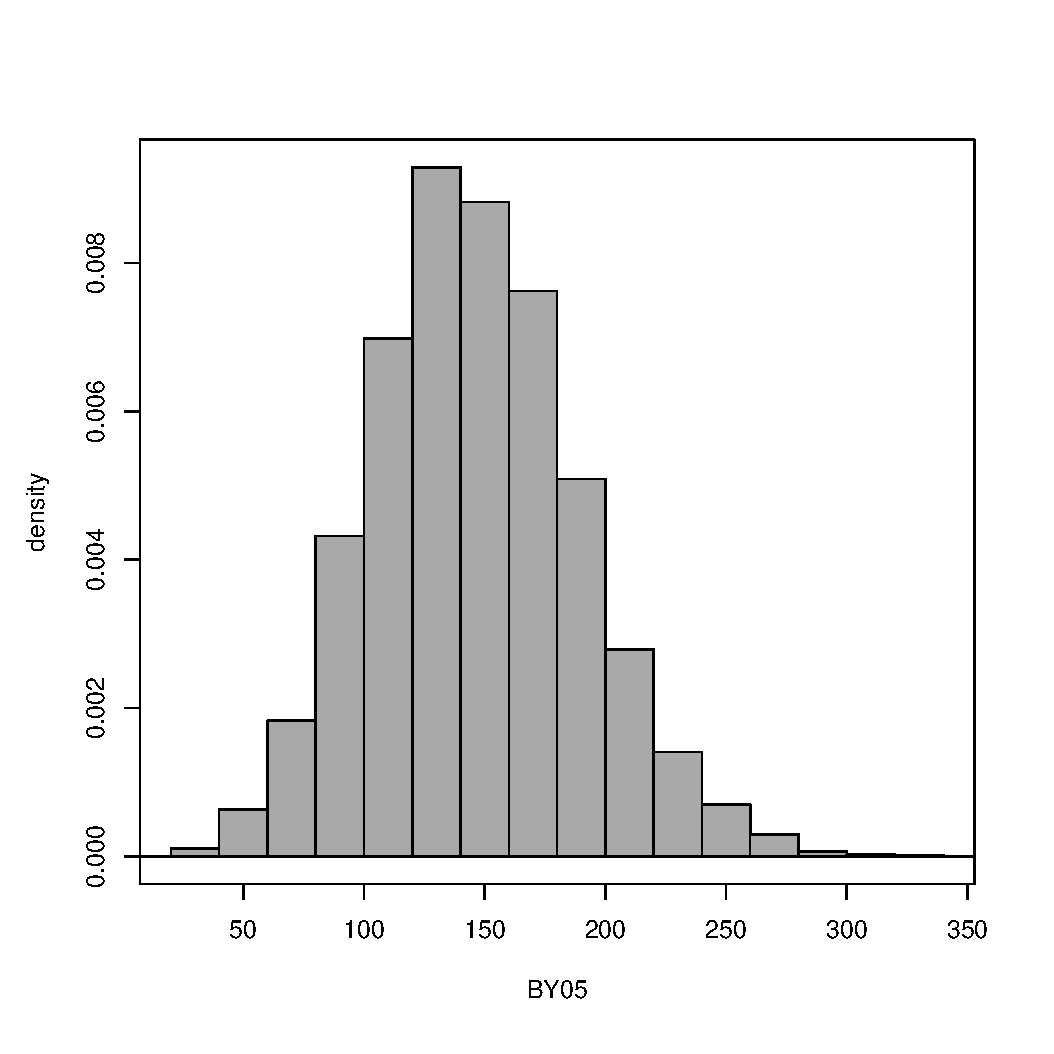
\includegraphics[width=\textwidth]{./CH11BY05}
\caption{}
\label{fig:CH11BY05}
\end{figure}

Our results have implications for how fish populations are monitored. If the interest is on the relative composition of the  mixed population overall, then most sampling programs will yield sufficient results. However, weak stocks are frequently a problem in conservation and fisheries management and precision of abundance estimates of smaller groups becomes important.  Obviously there is a tradeoff between sample size and number of subdivisions that can be supported. Previous work \cite{Gerritsen} shows this but the criteria for success is on overall (average) coverage. \citeasnoun{Thompson1987} found that a sample size of 510 should suffice under a worst case scenario for $\alpha=0.05$ (even proportions among groups but number of groups doesn't matter) as long as desired precision is expressed in absolute terms. If desired precision is expressed in relative terms (as we did), then no sample size will be sufficient as any of the group sizes approach zero. \citeasnoun{Steinhorst2010} in a study of Fall Chinook recommend that expected group sizes should be at least 300 to be confident in the estimates. For our Chinook estimates and simulation, 300 is large enough to ensure that we meet the NOAA sampling goals.  For the steelhead simulation, the smallest group size was 911 (BY04) and we met the NOAA sampling goal for all groups (Table \ref{table:SHsimresults}).  For the steelhead estimates (Table \ref{table:SHresults90}), we didn't meet the NOAA sampling goals for the groups of size 589 and 796 so clearly 300 is not adequate in this case. The next smallest group had 2218 fish (SFSALM) so on a relative basis 589 and 796 are ``small''.  Note that 796 is 36\% of 2218.  For the Chinook example, 259 (TUCANO)is 42\% of the next largest group 616 (CHMBLN).  From these results, it appears that we need to define ``small'' in relative rather than absolute terms.  Regardless of how we define small for a given data set, we must still decide if the ``lenient'' rule should apply.

In our scenario, sample size is a function of 1) total fish escapement, 2) trap sample rate, 3) handling rate, and 4) proportion wild. Total fish escapement and proportion wild are out of our hands, but sample size can be increased by increasing the trap sample rate and/or the handling rate. For SY2011 steelhead, the trap rate averaged 10\% and the average handling rate was slightly over 50\%. For Chinook salmon, the trap rate also averaged 10\% and the handling rate was about 75\%. We reran both the steelhead and Chinook salmon simulations increasing trap rates to 20\% and the handling rate to 100\%. This doubles the number of fish trapped in both cases. For steelhead, the number of fish for which sex, age, and stock was determined is 4 times the original simulation. For Chinook salmon, the number for which sex, age, and stock was determined is 2 2/3 times the original simulation. In practice, it is possible that this level of sampling would swamp the trapping crew (which can generally handle up to 800 fish a day due to logistical constraints), but we wanted to examine the effects of increasing sample sizes to this level. For both species, the percent half widths relative to the true population sizes were reduced in proportion to the reciprocal of the square root of the increase in sample size: $\sqrt{1/4} = 0.5$ for steelhead and $\sqrt{3/8} = 0.61$  for Chinook salmon.

In this study, we assumed that genetic stock was determined from IA without error and that accuracy and precision of genetic stock estimates was determined solely by variability in the trap and composition data sets. In reality, there is uncertainty in the determination of genetic stock for each fish. Uncertainty in genetic stock determination is related to the true genetic stock of origin of that individual and the relative genetic relatedness of that stock to all other genetic stocks present in the baseline; a fish may misallocate to a related genetic stock. Genetic stock misallocation may decrease the accuracy and precision of genetic stock estimates to an unknown degree. Accurate estimates of abundance by stock, and further, estimates of abundance by sex and by age within a stock would allow researchers to generate brood tables for each genetic stock. Brood tables summarize the number of offspring that return as adults in subsequent years for a given spawn or brood year (recruits per female or recruits per spawner) and provide a metric of productivity. Time-series estimates of recruits per spawner allow us to fit stock-recruitment curves, an important tool in fisheries management and conservation \cite{Ricker1973,Hilborn2003}. Further research will evaluate the uncertainty in genetic stock abundance estimates due to genetic misallocation and determine bias and precision of estimates of stock-sex and stock-age combinations.

Although our case study is characterized by a high degree of sampling control (near census of fish numbers with systematic compositional samples), there are lessons for other fisheries applications. Certainly SY2011 had more control than other years at Lower Granite Dam in that the run was as expected and there were no unexpected gaps in sampling. Frequently, sampling rate changes due to logistical concerns (e.g., more fish than expected can overwhelm trap and processing capacity) or environmental issues such as high summer water temperatures which can prohibit fish handling due to stress concerns. These types of problems will be greater in other cases where total abundance estimates have considerable variance or the sampling rate of the population for compositional data is small or unknown. The value of our case study is that it provides a best-case scenario for compositional analysis based on direct sampling.

In short, the two data set bootstrap method for finding confidence intervals worked well. Our method for estimating numbers of steelhead and spring/summer Chinook salmon in compositional groups provides unbiased estimators and confidence intervals with good coverages.

%% HERE WE DECLARE THE BIBLIOGRAPHYSTYLE TO USE AND THE BIBLIOGRAPHY DATABASE
\bibliographystyle{ECA_jasa}
\bibliography{RRrefs}

\end{document}